% !TEX program = pdflatex
% !TEX encoding = UTF-8 Unicode

\documentclass[
    aspectratio=169,
    12pt,
]{beamer}

\geometry{papersize={10in, 5.6in}}
% \geometry{papersize={8in, 4.5in}}

\setbeamertemplate{navigation symbols}{}
\usepackage{xcolor}
\definecolor{seeblau}{HTML}{00A9E0}
\setbeamercolor{structure}{fg=seeblau}


\usepackage[english]{babel}
\parskip=20pt

\usepackage{graphicx}
\usepackage{amsmath}
\usepackage{amssymb}
\usepackage{physics}
\usepackage[T1]{fontenc}
\usepackage[utf8]{inputenc}
\usepackage{markdown}

\usepackage[sfdefault]{roboto}
% \usepackage[sfdefault]{arimo}
% \usepackage[sfdefault]{FiraSans}
% \usepackage{libertinust1math} \usefonttheme[onlymath]{serif}

% emphasize by bold
\renewcommand{\emph}[1]{\textbf{#1}}

% make section frames
\newcommand{\sectionframe}{
    \begin{frame}
        \tableofcontents[currentsection]
    \end{frame}
}

\newcommand{\subsectionframe}{
    \begin{frame}
        \tableofcontents[currentsubsection]
    \end{frame}
}

% define full graphics command
\newcommand{\fullgraphic}[1]{
    \begin{figure}[H]
        \begin{center}
            \includegraphics[width=\textwidth, height=.85\textheight, keepaspectratio]{#1}
        \end{center}
    \end{figure}
}



\title{Optical signature of magnetic phase transitions in transition metal thiophosphates}
\subtitle{Batchelor Thesis}
\author{Leon Oleschko}
\date{\today}

\begin{document}

\begin{frame}
    \centering
    \Huge\color{seeblau}
    Optical signature of magnetic phase transitions\\ in transition metal thiophosphates
    \\\vspace{.5cm}
    \large \color{black}
    Bachelor Thesis of Leon Oleschko\\
    supervised by Dr. Mateusz Goryca
    \\
    \vspace{.5cm}
    \normalsize
    \today
    \vfill
    \begin{columns}
        \begin{column}{.3\textwidth}
            \centering
            
\includegraphics[width=\textwidth]{../figures/logo/UniKonstanz_Logo.pdf}
        \end{column}
        \begin{column}{.3\textwidth}
            \centering
            
\includegraphics[width=\textwidth]{../figures/logo/UniWarsaw.png}            
        \end{column}
    \end{columns}
\end{frame}

\section{Literature Review: Oct 2023}
\sectionframe

\begin{frame}{Search Terms}
	\begin{itemize}
		\item transition metal phosphor sulfates OR FePS3 OR NiPS3 OR CrPS4 OR MnPS3
		\item spectroscopy of transition metal phosphor sulfates OR FePS3 OR NiPS3 OR CrPS4 for magnetic field
		\item magnetic order OR magnetic phase in semiconductor AND spectroscopy
		\item kerr OR moke OR Magnetic Circular Dichroism Spectroscopy
	\end{itemize}
\end{frame}

\begin{frame}{Magnetic Structure and Metamagnetic Transitions in the van der Waals Antiferromagnet \textbf{CrPS4} - 1/3}
	\begin{columns}
		\column{.5\textwidth}
		\fullgraphic{phase_diagram.png}
		\small
		\par{A-AFM:} $\vec{m} \parallel \vec{n}_\text{lattice}=\vec{c}$
		\par{C-AFM:} $\vec{m} \nparallel \vec{c}$ (canted)
		\column{.2\textwidth}
		\fullgraphic{image1.png}
	\end{columns}

\end{frame}

\begin{frame}{Magnetic Structure and Metamagnetic Transitions in the van der Waals Antiferromagnet CrPS4 - 2/3}
	\begin{columns}
		\column{0.6\textwidth}
		\fullgraphic{image3.png}
		\column{.15\textwidth}
		\fullgraphic{image1.png}
		\column{.3\textwidth}
		$\theta=\measuredangle(\vec c, \vec H)$ is important!
		\\\vspace{1em}
		$\chi(B\approx 0, T\approx 0)\approx 0$ is a property of AFM?
		\\ \vspace{1em}
		A-AFM -- C-AFM transition based on $\dv{M}{H}$ (b)
	\end{columns}
\end{frame}

\begin{frame}{Magnetic Structure and Metamagnetic Transitions in the van der Waals Antiferromagnet CrPS4 - 3/3 Torque}
	\begin{columns}
		\column{0.7\textwidth}
		\fullgraphic{image4.png}
		\column{.3\textwidth}
		C-AFM -- FM transition based on $\dv[2]{\text{Torque}}{H}$ (a,b)
	\end{columns}
\end{frame}

\begin{frame}{Magnetism in the layered transition-metal thiophosphates MPS3}
	\begin{columns}
		\column{0.6\textwidth}
		\fullgraphic{image10.png}
	\column{.4\textwidth}
		Heisenberg model $\Rightarrow$ different splitting for different $\measuredangle(\vec H, \vec n)$
	\end{columns}
\end{frame}

\begin{frame}{Magnetization Study of the AFM-FM Coexistence in the Manganite System Pr$_\text{0.5}$Ca$_\text{0.5-x}$Sr$_\text{x}$MnO$_3$}
	Coexistence of AFM in the bulk interior and FM at the surface\\
	$\Rightarrow$ Different behaviour in Kerr (surface) and Faraday?

	\vspace{1em}
	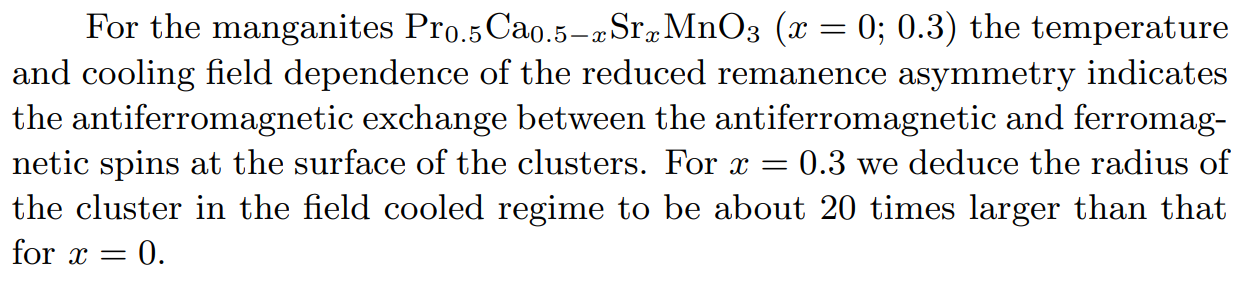
\includegraphics[width=\textwidth]{image5.png}
\end{frame}

\begin{frame}
	\textcolor{seeblau}{Field-dependent magneto-optical Kerr effect spectroscopy applied to the magnetic component diagnosis of a rubrene/Ni system}
	\begin{columns}
		\column{.5\textwidth}
		\fullgraphic{image6.png}
		\column{.4\textwidth}
		\small
		Rubrene: organic semiconductor
		\\ \vspace{1em}
		\fullgraphic{image7.png}
	\end{columns}
\end{frame}

\begin{frame}{Magnetic Order and Symmetry in the 2D Semiconductor CrSBr}
	\begin{columns}
		\column{0.7\textwidth}
		\fullgraphic{image9.png}
	\end{columns}
\end{frame}
\section{Current Status}
\sectionframe

\subsection{Materials}
\begin{frame}{Magnetism in van der Waals materials}
	\begin{columns}
		\column{.7\textwidth}
		\centering
		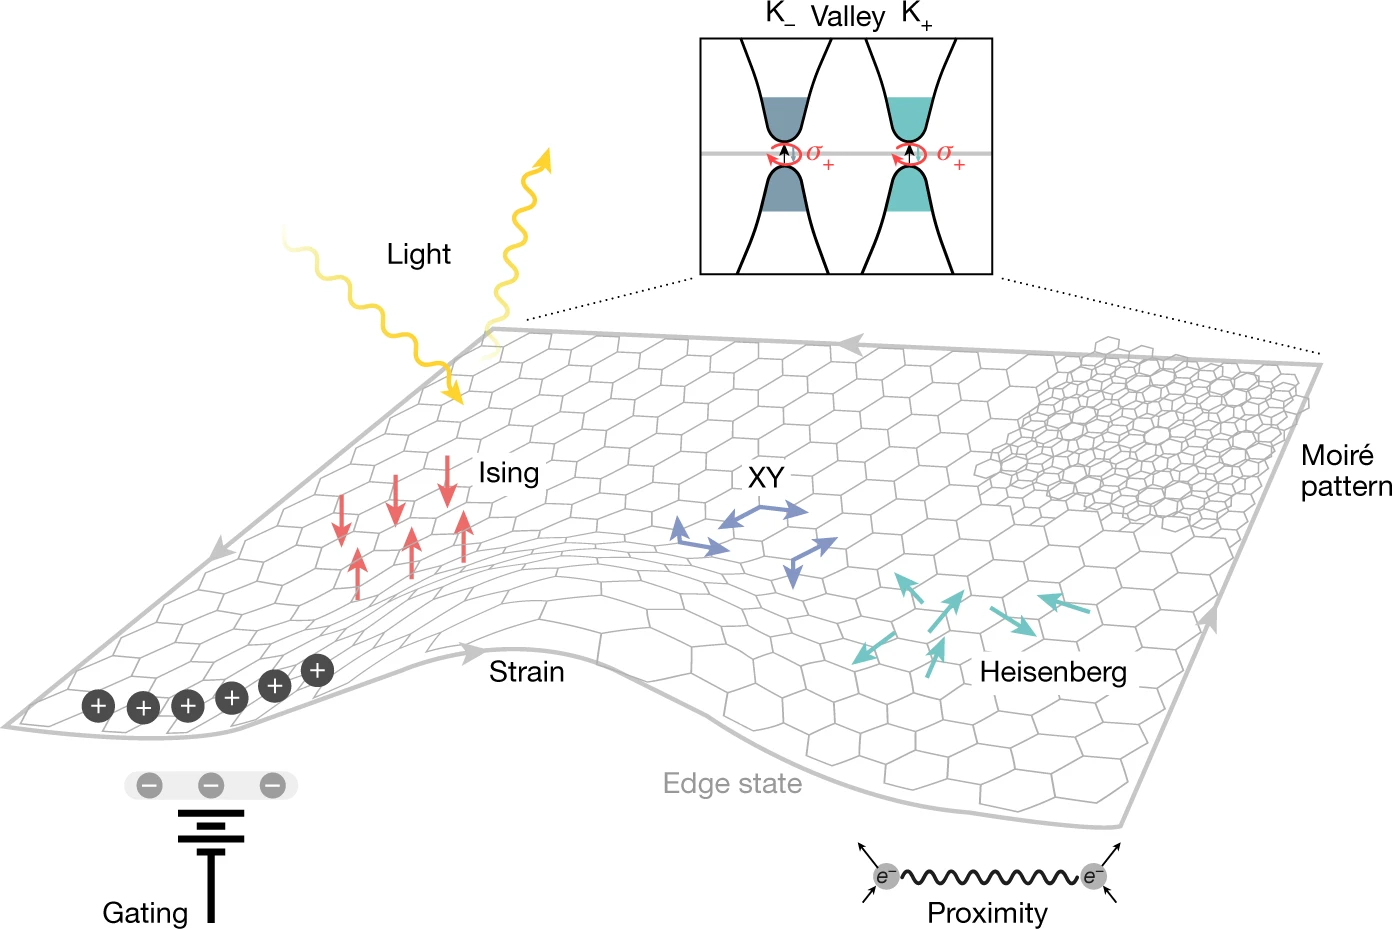
\includegraphics[width=\textwidth]{image11.png}\\
		\small\raggedleft Magnetism in two-dimensional van der Waals materials, Nature 2018

		\column{.3\textwidth}
		"While \emph{MnPS3} is best described by the \emph{isotropic Heisenberg Hamiltonian}, \\
		\emph{FePS3} is most effectively treated by the \emph{Ising model}, \\
		while \emph{NiPS3} is best described by the \emph{anisotropic Heisenberg Hamiltonian}."\\
		\vspace{1cm}
		\small\raggedleft
		Magnetism in the layered transition-metal thiophosphates MPS3 (M =Mn, Fe, and Ni), Physical Review B 1992
	\end{columns}
\end{frame}

\begin{frame}{NiPS$_3$}
	\centering
	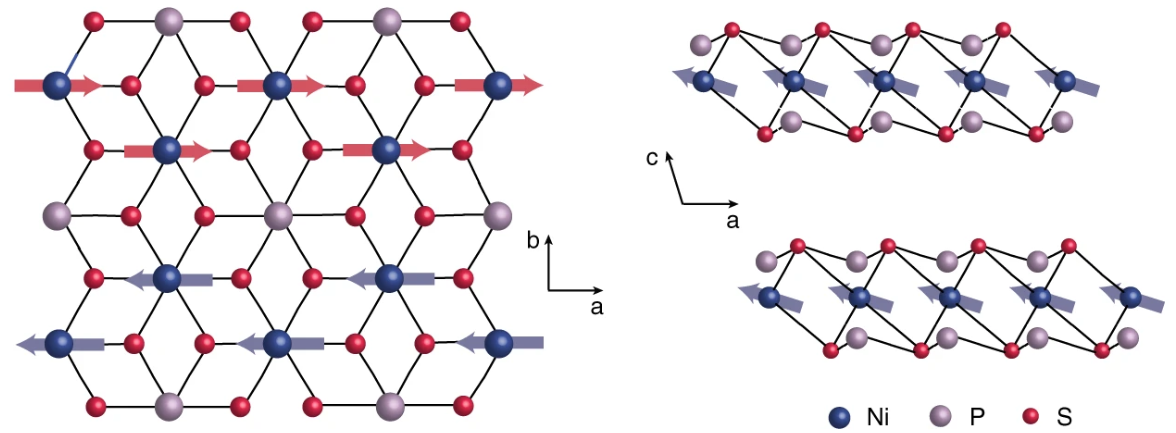
\includegraphics[width=.8\textwidth]{image13.png}
	\\\vspace{1cm}
	\small\raggedleft
	Exciton-driven antiferromagnetic metal in a correlated van der Waals insulator,
	Nature Communications 2021
\end{frame}

\subsection{Setup}
\begin{frame}{Setup}
	\centering
	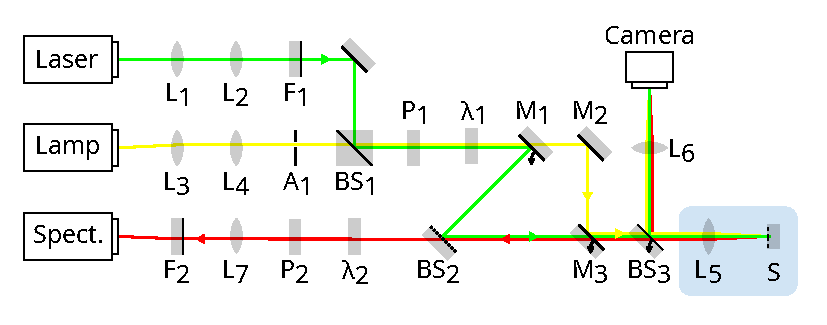
\includegraphics{../figures/setup.pdf}
\end{frame}


\subsection{Photoluminescence and Reflection at 0 T}
\begin{frame}{bulk PL spectra at 10 K}
	\centering
	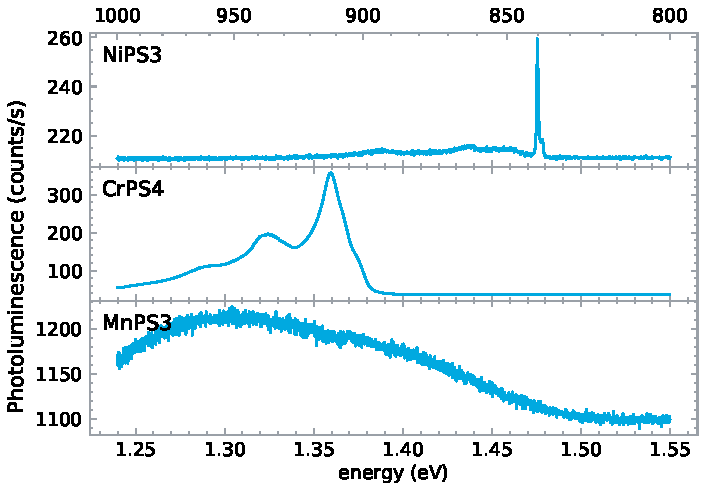
\includegraphics{../figures/2023-12-10 Combined PL.pdf}
\end{frame}

\begin{frame}{Reflectance spectra}
	\centering
	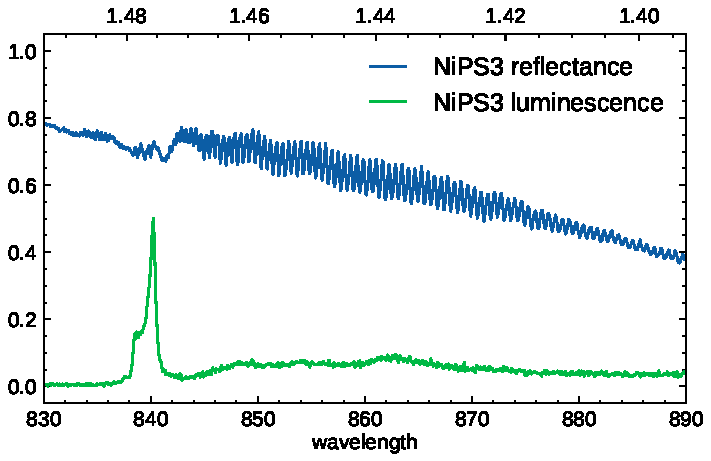
\includegraphics{../figures/2023-12-10 reflectance.pdf}
\end{frame}

\begin{frame}
	\begin{columns}
		\column{.3\textwidth}
		\centering
		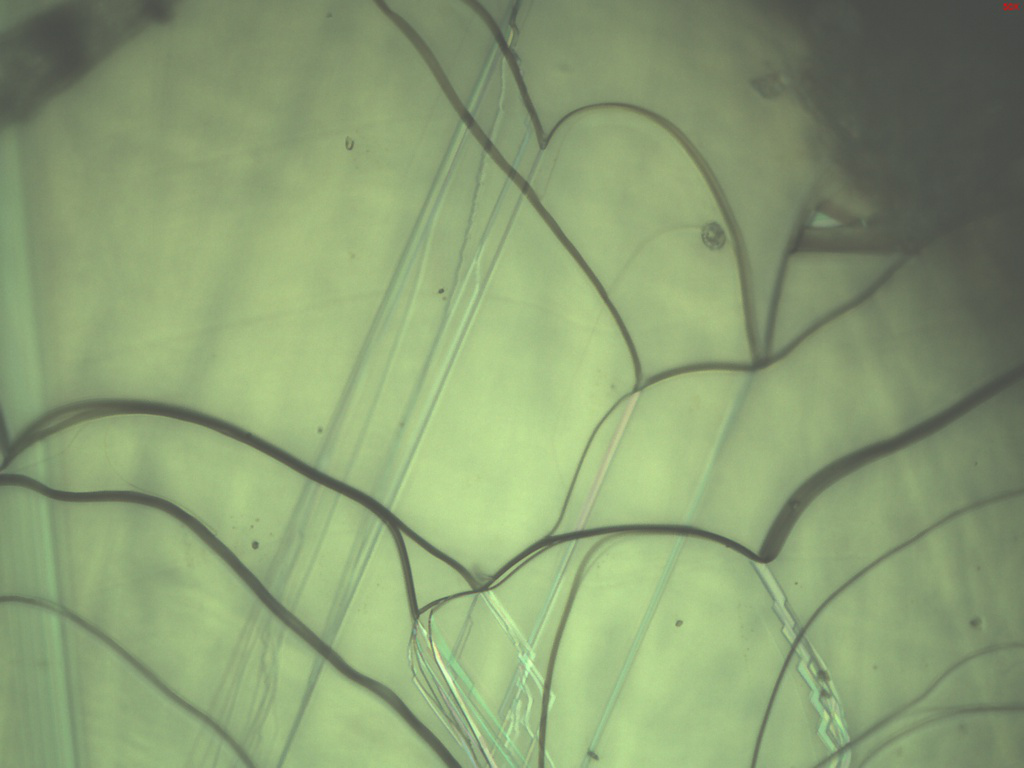
\includegraphics[width=\textwidth]{../figures/sample_photos/i001_MnPS3_50x_a.png}
		MnPS$_3$ Bulk Crystal (50x)

		\column{.3\textwidth}
		\centering
		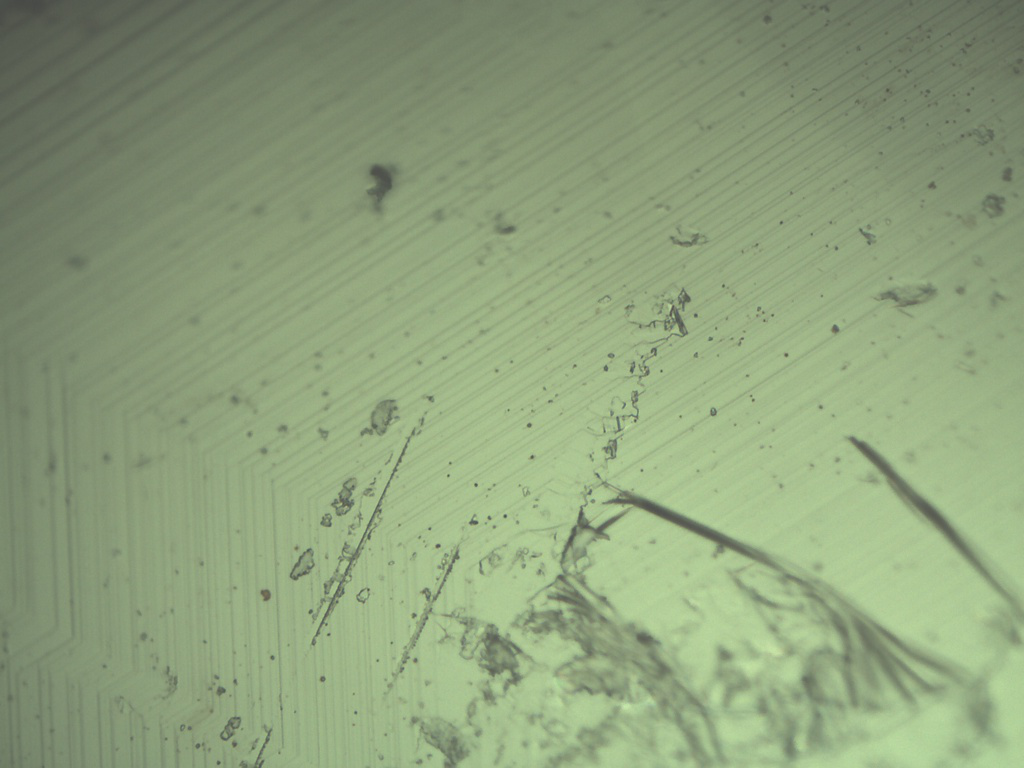
\includegraphics[width=\textwidth]{../figures/sample_photos/i005_NiPS3_50x.png}
		NiPS$_3$ Bulk Crystal (50x)

		\column{.3\textwidth}
		\centering
		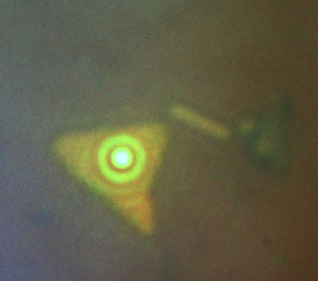
\includegraphics[width=\textwidth]{../figures/sample_photos/exfoliated_NiPS3.png}
		NiPS$_3$ Exfoliated Crystal
	\end{columns}

\end{frame}


\subsection{NiPS$_3$ in magnetic field}
\subsubsection{in plane}
\subsectionframe

\begin{frame}{Instability of the Lens assembly?}
	\begin{columns}
		\column{.6\textwidth}
		\centering
		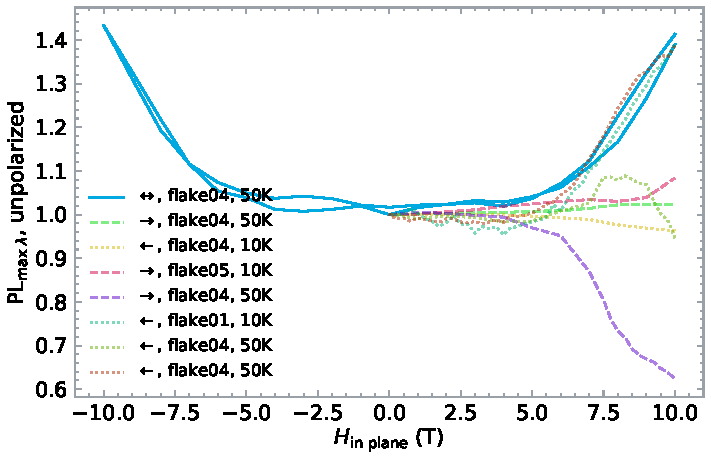
\includegraphics{../figures/2023-12-10 lens movement.pdf}

		\column{.3\textwidth}
		\begin{figure}
			\centering
			\includegraphics[width=\textwidth]{../figures/sampleHolder.pdf}
			Field in plane of the image.
		\end{figure}
	\end{columns}
\end{frame}

\begin{frame}{Splitting of the PL peak at $\measuredangle P,H=0$}
	\begin{columns}
	\column{.5\textwidth}
	\centering
	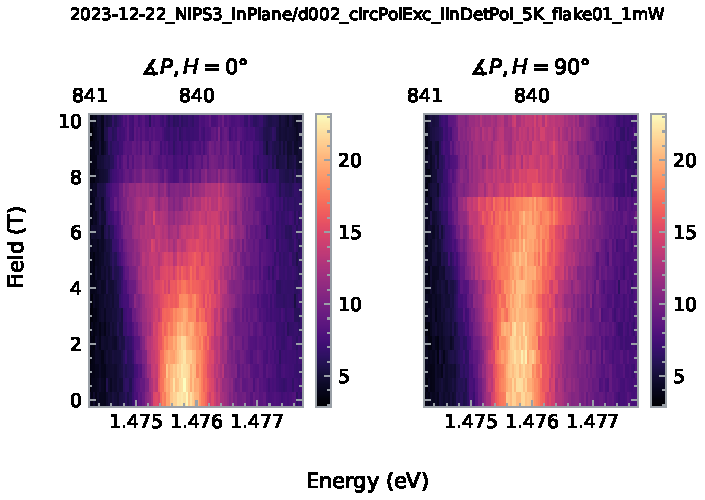
\includegraphics{../figures/2023-12-10 splitting.pdf}
	\column{.5\textwidth}
	\centering
	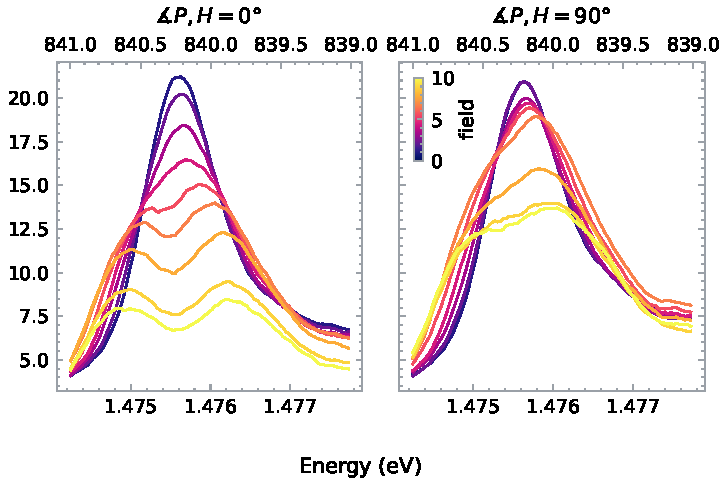
\includegraphics{../figures/2023-12-10 splitting quantified.pdf}
	\end{columns}
\end{frame}


\begin{frame}{Polarisation}
	\centering
	% 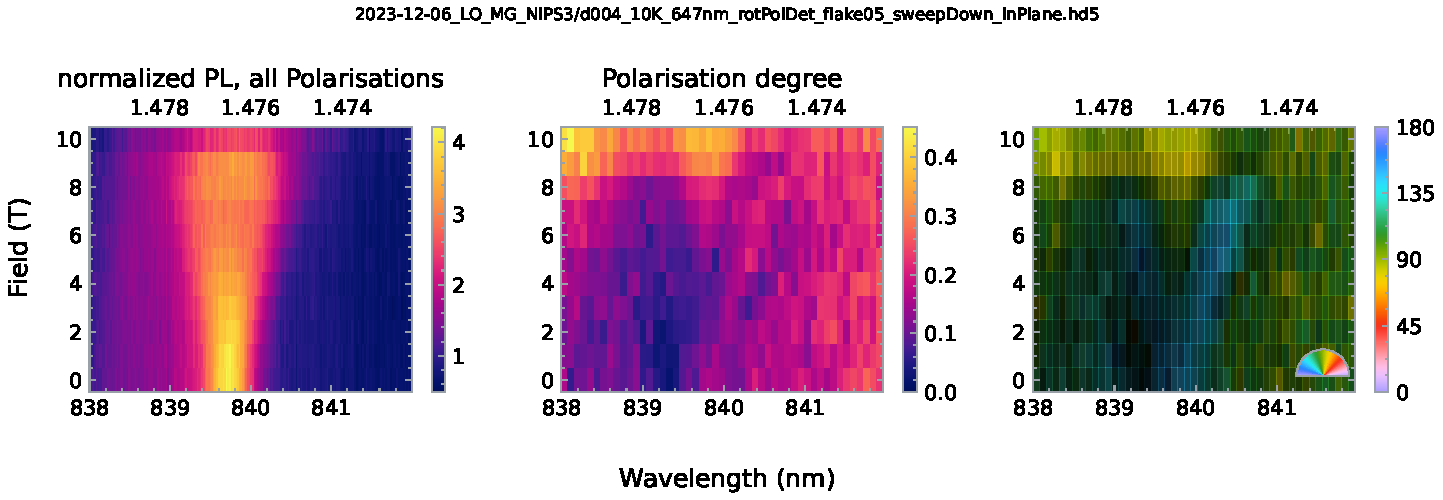
\includegraphics{../figures/2023-12-10 splitting polarisation on 2023-12-06_LO_MG_NiPS3 d004_10K_647nm_rotPolDet_flake05_sweepDown_inPlane.hd5.pdf}
	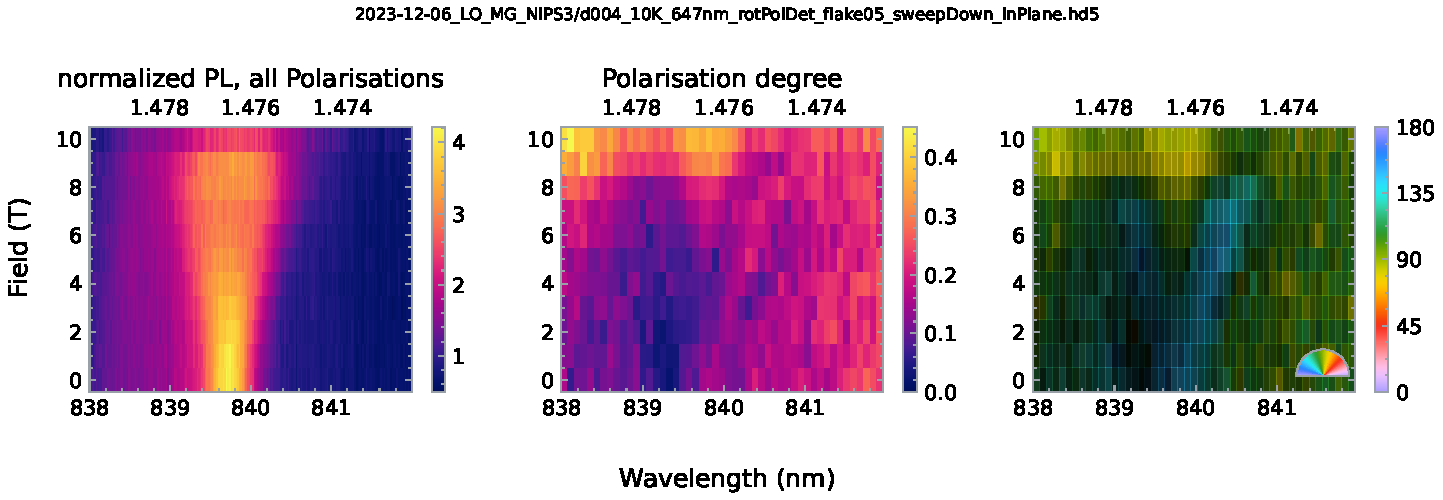
\includegraphics{../figures/2023-12-10 splitting polarisation on 2023-12-06_LO_MG_NiPS3 d004_10K_647nm_rotPolDet_flake05_sweepDown_inPlane.hd5.pdf}
\end{frame}
\begin{frame}{at 50K}
	\centering
	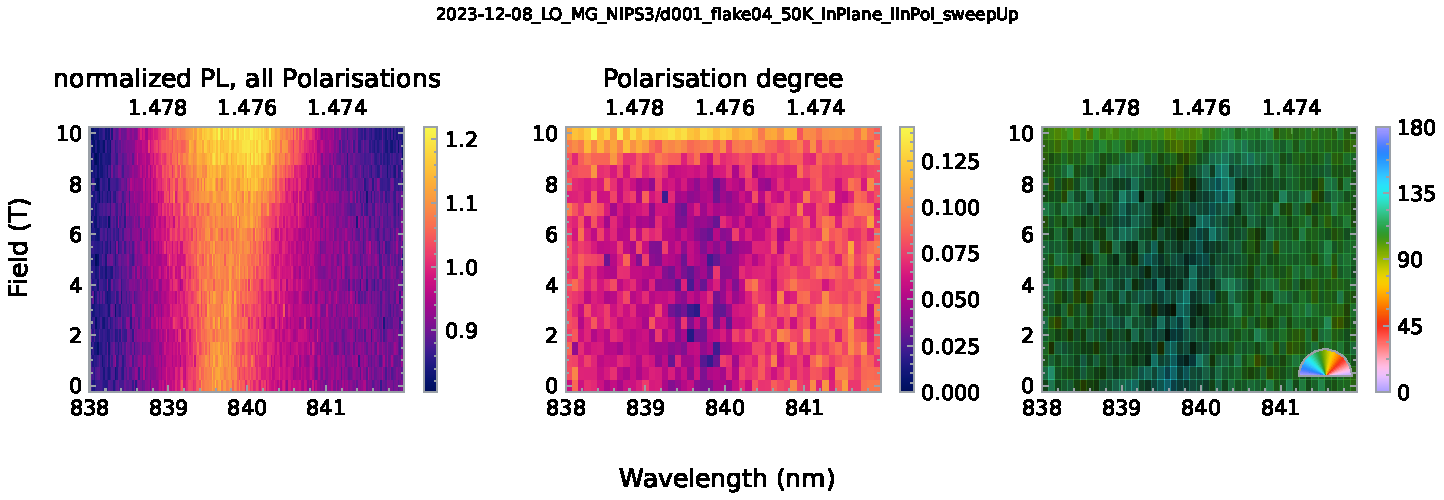
\includegraphics{../figures/2023-12-10 splitting polarisation on 2023-12-08_LO_MG_NiPS3 d001_flake04_50K_inPlane_linPol_sweepUp.pdf}
\end{frame}

\begin{frame}{Understanding in Plane field}
	\begin{columns}
		\column{.3\textwidth}
		My measurement:\\\vspace{1cm}
		\centering
		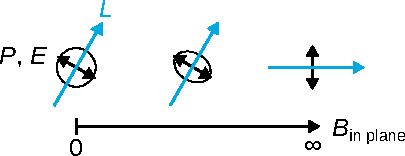
\includegraphics{../figures/vector_rotation.pdf}
		\\\vspace{1cm}\raggedleft\small
		Based on Fig. 4 b in Spin-induced linear polarization of photoluminescence in antiferromagnetic van der Waals crystals, Nature Materials 2021
		\column{.7\textwidth}
		\centering
		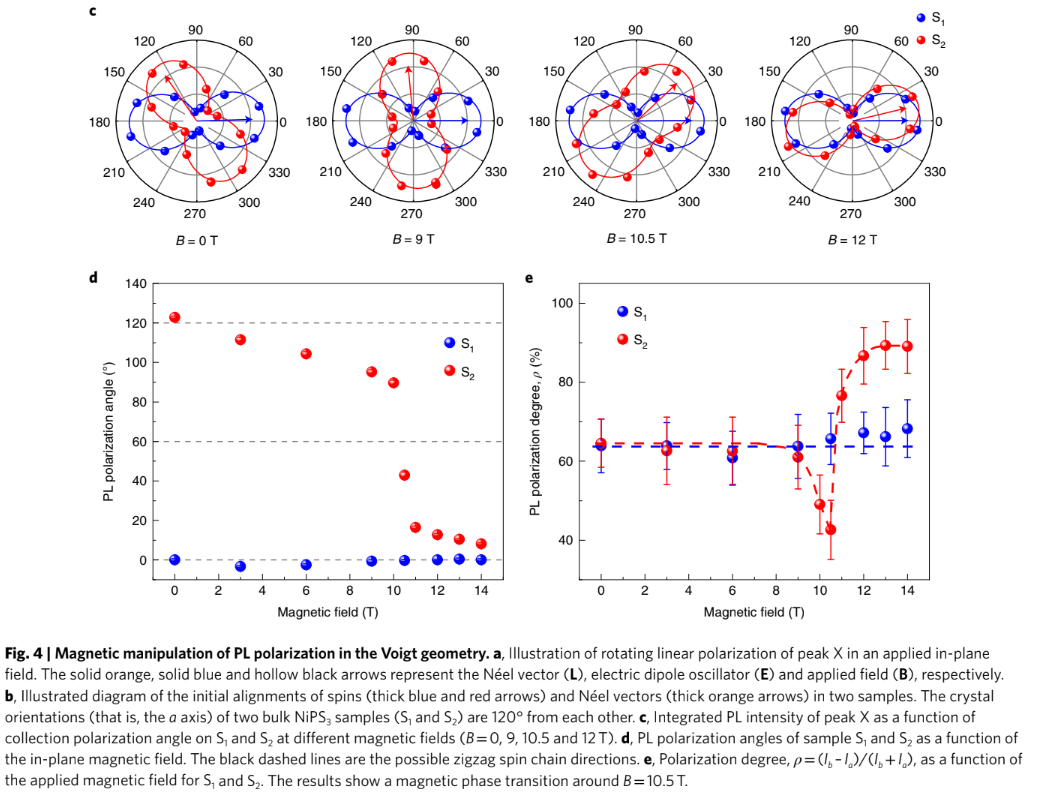
\includegraphics[width=\textwidth]{image12.png}

	\end{columns}
\end{frame}

\subsubsection{out of plane}
\begin{frame}{Out of plane field}
	\centering
	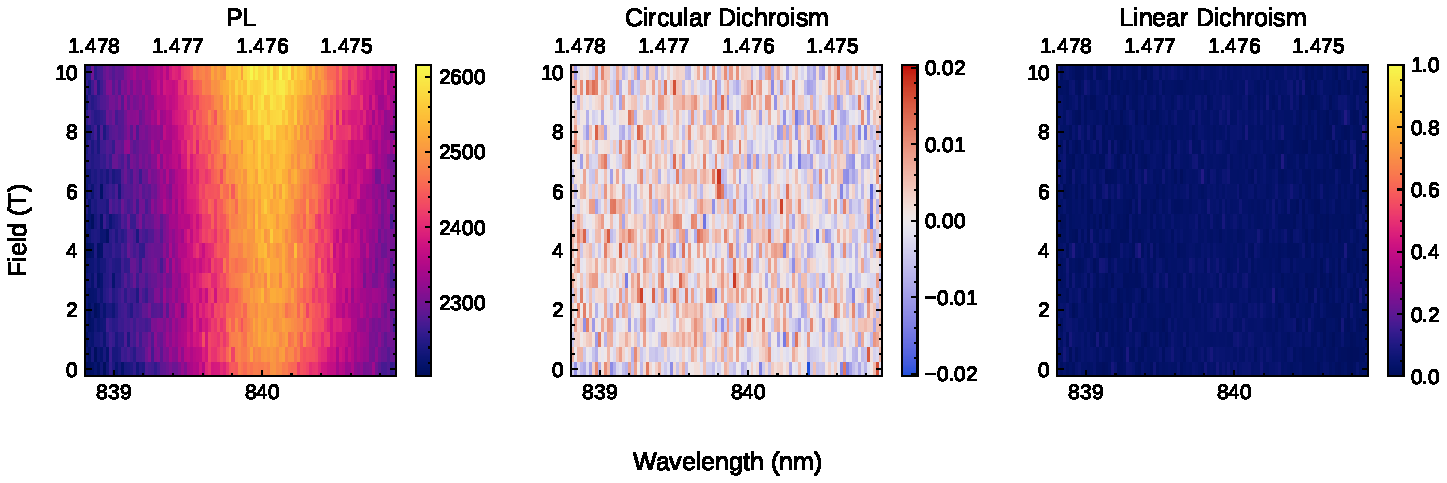
\includegraphics{../figures/2023-12-10 circular dichroism 2023-12-11_NiPS3 d002_flake04_50K_circPol_inPlane.pdf}
\end{frame}

\subsection{CrPS$_4$}
\subsectionframe

\begin{frame}{excitation power dependence}
	\centering
	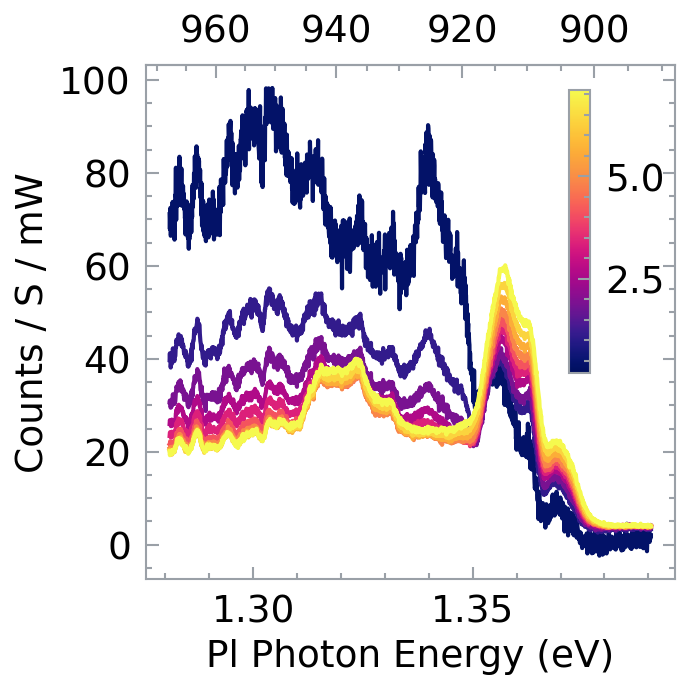
\includegraphics{../figures/2023-12-14 CrPS4 excitation power dependence.png}
\end{frame}

\begin{frame}{CrPS$_4$: $CD \propto M$ ?}
	\begin{columns}
		\column{.5\textwidth}
		My measurement:\\
		\centering
		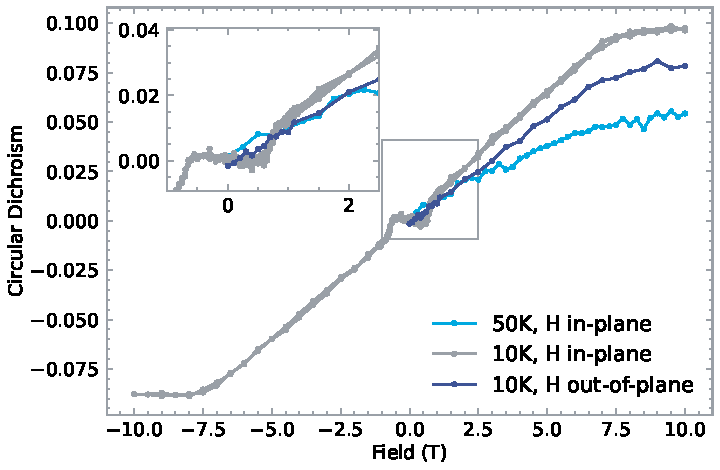
\includegraphics{../figures/2023-12-14 CrPS4 circular dichroism.pdf}
	
		\column{.5\textwidth}
		\centering
		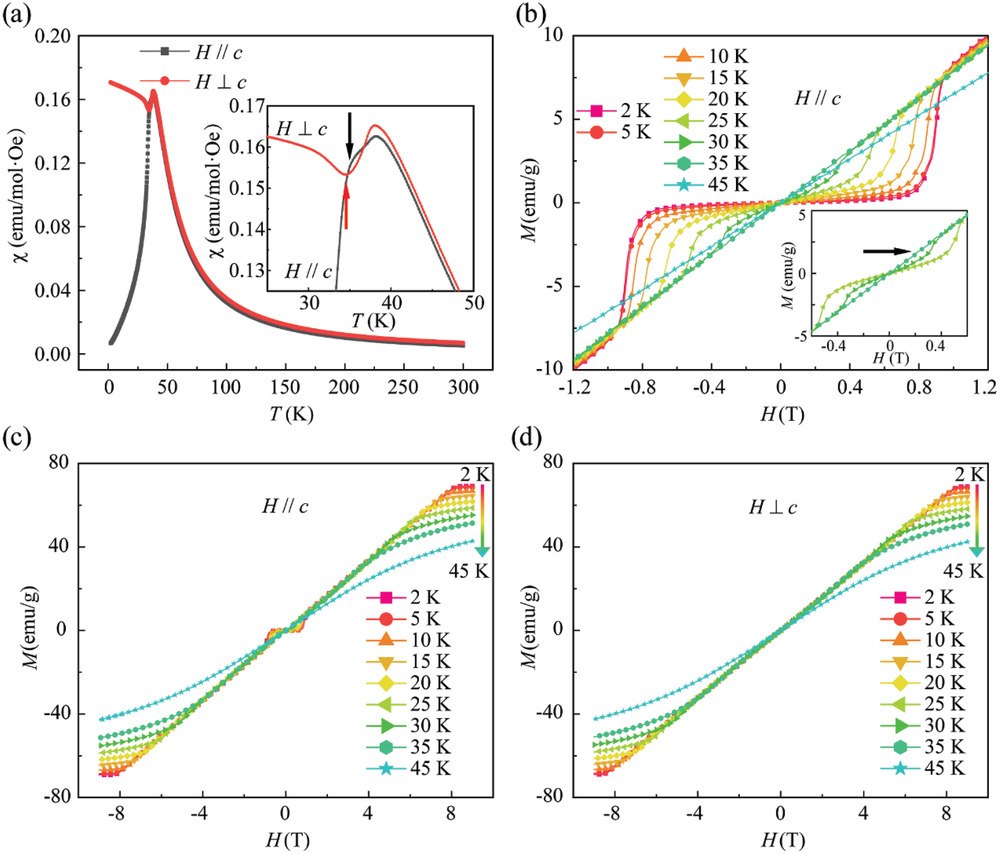
\includegraphics[width=\textwidth]{image14.png}
		\\\vspace{1cm}\raggedright\small
		Magnetic Structure and Metamagnetic Transitions in the van der Waals
		Antiferromagnet CrPS$_4$, Advanced Materials 2020

	\end{columns}
	
\end{frame}


\begin{frame}{moving flakes}
	\begin{columns}

		\column{.5\textwidth}
		\centering
		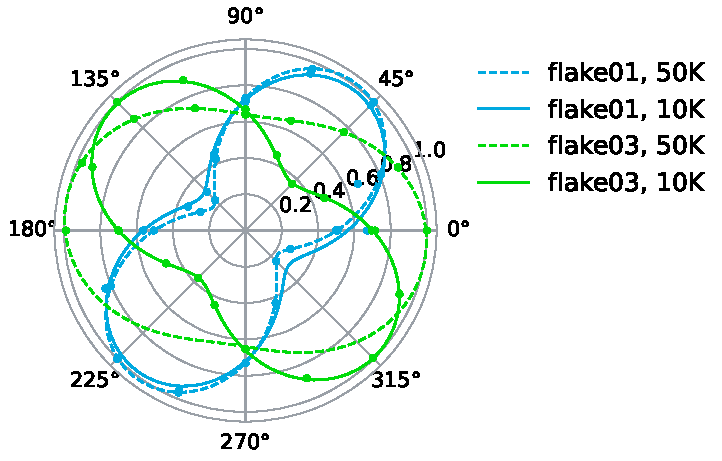
\includegraphics{../figures/2023-12-14 flake turning linear polarisation.pdf}


		\column{.5\textwidth}
		\centering
		\begin{figure}
			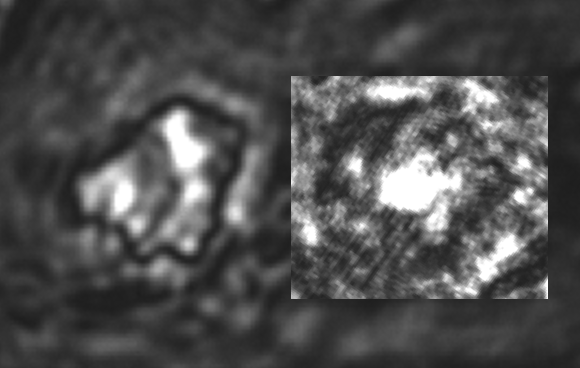
\includegraphics[width=\textwidth]{../../data/2023-12-14_CrPS4_outPlane/flake03_rotation_cropped.png}
			\caption{Flake 03, background: flake after cooldown, foreground: flake before, rotated by 30°}
		\end{figure}
	\end{columns}

\end{frame}

\begin{frame}{Linear Polarisation}
	\centering
	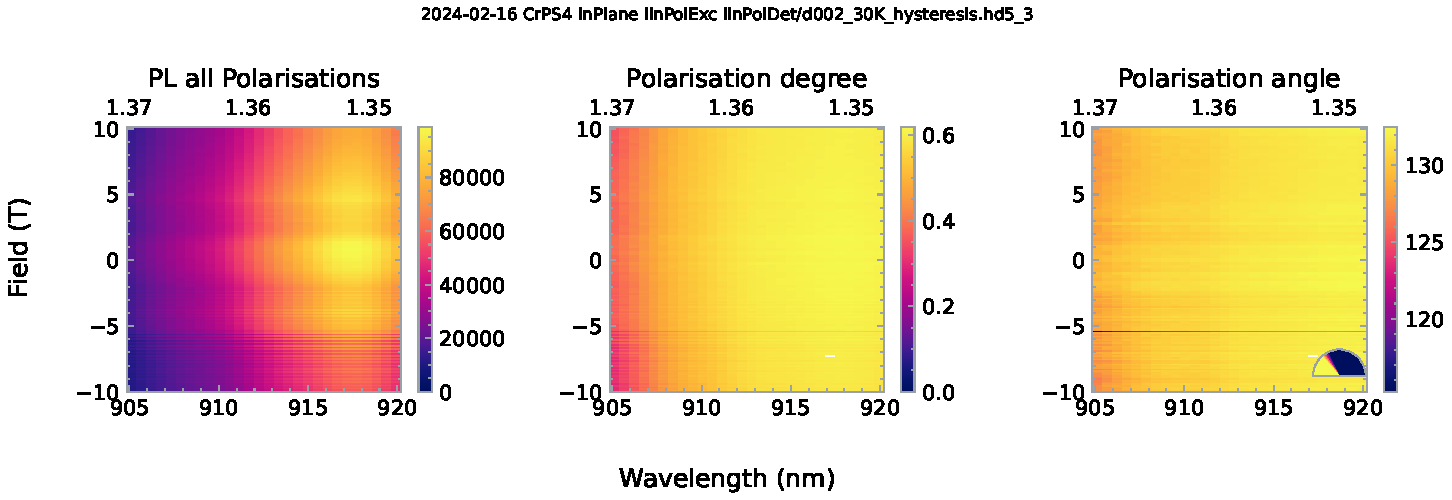
\includegraphics{../figures/2023-12-15 CrPS4 linear dichroism.pdf}
\end{frame}


\section{Writing}
\sectionframe


\begin{frame}
\end{frame}

% \appendix

% \section{Literature Review: Oct 2023}
\sectionframe

\begin{frame}{Search Terms}
	\begin{itemize}
		\item transition metal phosphor sulfates OR FePS3 OR NiPS3 OR CrPS4 OR MnPS3
		\item spectroscopy of transition metal phosphor sulfates OR FePS3 OR NiPS3 OR CrPS4 for magnetic field
		\item magnetic order OR magnetic phase in semiconductor AND spectroscopy
		\item kerr OR moke OR Magnetic Circular Dichroism Spectroscopy
	\end{itemize}
\end{frame}

\begin{frame}{Magnetic Structure and Metamagnetic Transitions in the van der Waals Antiferromagnet \textbf{CrPS4} - 1/3}
	\begin{columns}
		\column{.5\textwidth}
		\fullgraphic{phase_diagram.png}
		\small
		\par{A-AFM:} $\vec{m} \parallel \vec{n}_\text{lattice}=\vec{c}$
		\par{C-AFM:} $\vec{m} \nparallel \vec{c}$ (canted)
		\column{.2\textwidth}
		\fullgraphic{image1.png}
	\end{columns}

\end{frame}

\begin{frame}{Magnetic Structure and Metamagnetic Transitions in the van der Waals Antiferromagnet CrPS4 - 2/3}
	\begin{columns}
		\column{0.6\textwidth}
		\fullgraphic{image3.png}
		\column{.15\textwidth}
		\fullgraphic{image1.png}
		\column{.3\textwidth}
		$\theta=\measuredangle(\vec c, \vec H)$ is important!
		\\\vspace{1em}
		$\chi(B\approx 0, T\approx 0)\approx 0$ is a property of AFM?
		\\ \vspace{1em}
		A-AFM -- C-AFM transition based on $\dv{M}{H}$ (b)
	\end{columns}
\end{frame}

\begin{frame}{Magnetic Structure and Metamagnetic Transitions in the van der Waals Antiferromagnet CrPS4 - 3/3 Torque}
	\begin{columns}
		\column{0.7\textwidth}
		\fullgraphic{image4.png}
		\column{.3\textwidth}
		C-AFM -- FM transition based on $\dv[2]{\text{Torque}}{H}$ (a,b)
	\end{columns}
\end{frame}

\begin{frame}{Magnetism in the layered transition-metal thiophosphates MPS3}
	\begin{columns}
		\column{0.6\textwidth}
		\fullgraphic{image10.png}
	\column{.4\textwidth}
		Heisenberg model $\Rightarrow$ different splitting for different $\measuredangle(\vec H, \vec n)$
	\end{columns}
\end{frame}

\begin{frame}{Magnetization Study of the AFM-FM Coexistence in the Manganite System Pr$_\text{0.5}$Ca$_\text{0.5-x}$Sr$_\text{x}$MnO$_3$}
	Coexistence of AFM in the bulk interior and FM at the surface\\
	$\Rightarrow$ Different behaviour in Kerr (surface) and Faraday?

	\vspace{1em}
	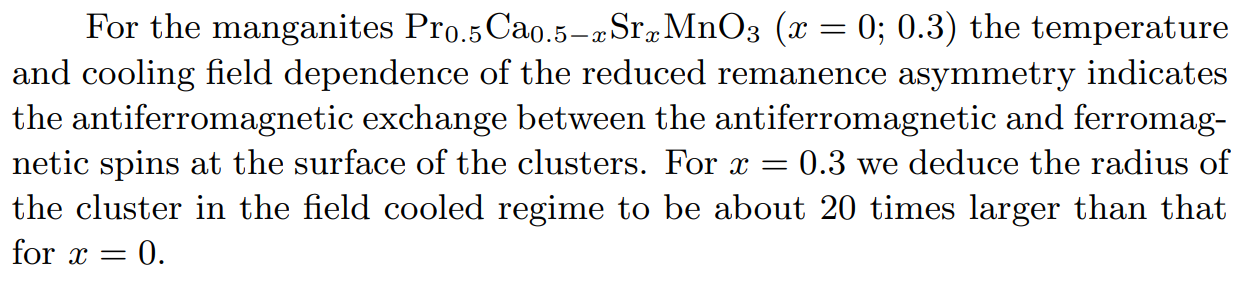
\includegraphics[width=\textwidth]{image5.png}
\end{frame}

\begin{frame}
	\textcolor{seeblau}{Field-dependent magneto-optical Kerr effect spectroscopy applied to the magnetic component diagnosis of a rubrene/Ni system}
	\begin{columns}
		\column{.5\textwidth}
		\fullgraphic{image6.png}
		\column{.4\textwidth}
		\small
		Rubrene: organic semiconductor
		\\ \vspace{1em}
		\fullgraphic{image7.png}
	\end{columns}
\end{frame}

\begin{frame}{Magnetic Order and Symmetry in the 2D Semiconductor CrSBr}
	\begin{columns}
		\column{0.7\textwidth}
		\fullgraphic{image9.png}
	\end{columns}
\end{frame}

\begin{frame}
\end{frame}

\end{document}